\documentclass[12pt, letterpaper]{article}

% --- Packages ---
\usepackage{geometry}
 \geometry{margin=1in}
\usepackage{graphicx}
\usepackage{amsmath, amssymb}
\usepackage{booktabs}
\usepackage{hyperref}
\usepackage{cite}
\usepackage{setspace}
\onehalfspacing
\usepackage{fontspec}
\usepackage{polyglossia}
\usepackage{float}
\usepackage{svg}
\usepackage{enumitem}
\setmainlanguage{vietnamese}

\usepackage{listings}
\usepackage{xcolor}

\lstset{
    language=C,
    basicstyle=\ttfamily\small,
    keywordstyle=\color{blue},
    stringstyle=\color{red},
    commentstyle=\color{green!60!black},
    breaklines=true,
    frame=single, % Tạo khung xung quanh code
    backgroundcolor=\color{gray!5}
}

\renewcommand{\lstlistingname}{Mã nguồn}

% --- Metadata ---
\title{Bổ sung một hàm hệ thống mới vào nhân HĐH Ubuntu 24.04 và sử dụng hàm đó}
\author{Đỗ Hoàng Gia Bảo - 23020783 \\ \small Khoa Điện tử - Viễn Thông}
\date{\today}

\begin{document}

\maketitle

\begin{abstract}
Báo cáo sẽ trình bày các bước giải bài tập 1, 2 cuối slide "Bài 3-Lập lịch CPU"
\end{abstract}
% --- Front Matter (Roman Numerals) ---
\newpage
\tableofcontents

% --- Main Content (Arabic Numerals) ---
\newpage
\pagenumbering{arabic}
\setcounter{page}{3} % This automatically resets the counter to 1

\section{Các khái niệm}
\subsection{Biểu đồ Gantt}
Biểu đồ Gantt là một loại sơ đồ dùng để biểu diễn sự phân chia thời gian thực thi của các tiến trình trên CPU theo trục thời gian. Trong lập lịch CPU, biểu đồ Gantt giúp quan sát trực quan tiến trình nào đang chiếm giữ CPU tại mỗi thời điểm, từ đó xác định được thời điểm bắt đầu và thời điểm kết thúc của từng tiến trình.
\subsection{Thời gian chờ (Waiting time)}
Thời gian chờ ($T_w$) là tổng thời gian mà một tiến trình phải nằm trong hàng đợi sẵn sàng (ready queue) nhưng không được cấp phát CPU để thực thi. 
\[ T_w = \text{Thời gian hoàn thành (Turnaround time)} - \text{Thời gian chạy (Burst time)} \]
Đối với các thuật toán cho phép dừng (preemptive), thời gian chờ có thể tích lũy từ nhiều khoảng thời gian gián đoạn khác nhau.
\subsection{Thời gian phản hồi (Response Time)}
Thời gian phản hồi ($T_{res}$) là khoảng thời gian từ lúc tiến trình bắt đầu vào hàng đợi sẵn sàng cho đến khi nó nhận được CPU lần đầu tiên. Đây là chỉ số quan trọng trong các hệ thống tương tác để đánh giá độ nhạy của hệ điều hành.
\[ T_{res} = \text{Thời điểm bắt đầu chạy lần đầu} - \text{Thời gian đến} \]
\subsection{Thời gian hoàn thành (Turnaround Time)}
Thời gian hoàn thành ($T_{tt}$) là tổng thời gian tính từ lúc tiến trình được đưa vào hệ thống cho đến khi nó kết thúc hoàn toàn việc thực thi.
\[ T_{tt} = \text{Thời điểm kết thúc} - \text{Thời điểm đến} \]
Hoặc cũng có thể tính bằng: $T_{tt} = \text{Thời gian chờ} + \text{Thời gian chạy}$.
\subsection{Chuyển trạng thái của CPU}
Chuyển trạng thái là quá trình lưu lại trạng thái của tiến trình hiện tại (đang chạy) và nạp trạng thái của tiến trình tiếp theo từ hàng đợi sẵn sàng vào CPU.
\section{Bài tập 1}
\subsection{Đề bài}
Có 5 tiến trình $P_{1}$, $P_{2}$, $P_{3}$, $P_{4}$, $P_{5}$ với thời gian chạy CPU (ms), thời gian đến và số hiệu ưu tiên như sau:
\begin{table}[H]
    \centering
    \caption{Bảng thống kê thời gian chạy, số hiệu ưu tiên, thời gian đến của 5 tiến trình}
    \begin{tabular}{|c|c|c|c|}
        \hline
        & \textbf{Thời gian chạy} & \textbf{Số hiệu ưu tiên} & \textbf{Thời gian đến} \\
        \hline
        $P_{1}$ & 2 & 2 & 0 \\
        $P_{2}$ & 1 & 1 & 1 \\
        $P_{3}$ & 8 & 5 & 3 \\
        $P_{4}$ & 4 & 3 & 4 \\
        $P_{5}$ & 5 & 4 & 5 \\
        \hline
    \end{tabular}
\end{table}
\noindent Với mỗi thuật toán lập lịch sau hãy vẽ biểu đồ Gantt và tính thời gian chờ trung bình, thời gian
phản hồi trung bình, thời gian hoàn thành trung bình, số lần chuyển trạng thái của CPU.
\noindent Các thuật toán cần thực hiện:
\begin{enumerate}[label=\alph*.]
    \item Round Robin với quantum $q = 2$ (ms)
    \item SJF (Shortest Job First) cho phép dừng (Preemptive)
    \item Lập lịch theo số hiệu ưu tiên cho phép dừng (Ưu tiên cao hơn chạy trước)
\end{enumerate}
\subsection{Giải bài tập}
\subsubsection{Giải câu a}
Khi sử dụng thuật toán Round Robin với quantum q = 2(ms), các tiến trình sẽ được xử lý thể hiện trên biểu đồ Gantt như sau:
\begin{figure}[H]
    \centering 
    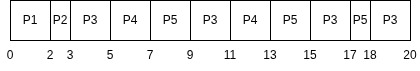
\includegraphics[width=0.8\textwidth]{image1.png}
    \caption{Biểu đồ Gantt cho thuật toán Round Robin với quantum q = 2 (ms)} 
    \label{fig:image1} 
\end{figure}
\noindent Từ biểu đồ Gantt, thời gian chờ trung bình, thời gian phản hồi trung bình, thời gian hoàn thành trung bình, số lần chuyển trạng thái của CPU được tính như sau:\\\\
\textbf{Thời gian chờ trung bình}
\begin{itemize}
    \item Thời gian chờ $T_{w1}$ = (2 - 0) - 2 = 0
    \item Thời gian chờ $T_{w2}$ = (3 - 1) - 1 = 1
    \item Thời gian chờ $T_{w3}$ = (20 - 3) - 8 = 9
    \item Thời gian chờ $T_{w4}$ = (13 - 4) - 4 = 5
    \item Thời gian chờ $T_{w5}$ = (18 - 5) - 5 = 8
    \item Thời gian chờ trung bình $T_w$ = $\frac{T_{w1} + T_{w2} + T_{w3} + T_{w4} + T_{w5}}{5} = \frac{0 + 1 + 9 + 5 + 8}{5} = 4.6 (ms)$ 
\end{itemize}
\textbf{Thời gian phản hồi trung bình}
\begin{itemize}
    \item Thời gian phản hồi $T_{res1}$ = 0 - 0 = 0
    \item Thời gian phản hồi $T_{res2}$ = 2 - 1 = 1
    \item Thời gian phản hồi $T_{res3}$ = 3 - 3 = 0
    \item Thời gian phản hồi $T_{res4}$ = 5 - 4 = 1
    \item Thời gian phản hồi $T_{res5}$ = 7 - 5 = 2
    \item Thời gian phản hồi trung bình $T_{res}$ = $\frac{T_{res1} + T_{res2} + T_{res3} + T_{res4} + T_{res5}}{5} = \frac{0 + 1 + 0 + 1 + 2}{5} = 0.8 (ms)$ 
\end{itemize}
\textbf{Thời gian hoàn thành trung bình}
\begin{itemize}
    \item Thời gian hoàn thành $T_{tat1}$ = 2 - 0 = 2
    \item Thời gian hoàn thành $T_{tat2}$ = 3 - 1 = 2
    \item Thời gian hoàn thành $T_{tat3}$ = 20 - 3 = 17
    \item Thời gian hoàn thành $T_{tat4}$ = 13 - 4 = 9
    \item Thời gian hoàn thành $T_{tat5}$ = 18 - 5 = 13
    \item Thời gian hoàn thành trung bình $T_{tat}$ = $\frac{T_{tat1} + T_{tat2} + T_{tat3} + T_{tat4} + T_{tat5}}{5} = \frac{2 + 2 + 17 + 9 + 13}{5} = 8.6 (ms)$ 
\end{itemize}
\textbf{Số lần chuyển trạng thái của CPU}
Dựa trên biểu đồ Gantt, vì mỗi một chuyển đổi từ tiến trình này sang tiến trình khác được tính là một chuyển trạng thái của CPU, số lần chuyển trạng thái là
\begin{itemize}
    \item Lần chuyển 1: $P_1 \rightarrow P_2$
    \item Lần chuyển 2: $P_2 \rightarrow P_3$
    \item Lần chuyển 3: $P_3 \rightarrow P_4$
    \item Lần chuyển 4: $P_4 \rightarrow P_5$
    \item Lần chuyển 5: $P_5 \rightarrow P_3$
    \item Lần chuyển 6: $P_3 \rightarrow P_4$
    \item Lần chuyển 7: $P_4 \rightarrow P_5$
    \item Lần chuyển 8: $P_5 \rightarrow P_3$
    \item Lần chuyển 9: $P_3 \rightarrow P_5$
    \item Lần chuyển 10: $P_5 \rightarrow P_3$
    \item Tổng số lần chuyển trạng thái: 10
\end{itemize}
\subsubsection{Giải câu b}
Khi sử dụng thuật toán SJF (Shortest Job First) cho phép dừng (Preemptive), các tiến trình sẽ được xử lý thể hiện trên biểu đồ Gantt như sau:
\begin{figure}[H]
    \centering 
    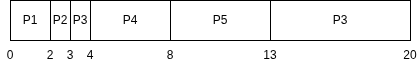
\includegraphics[width=0.8\textwidth]{image2.png}
    \caption{Biểu đồ Gantt cho thuật toán SJF} 
    \label{fig:image2} 
\end{figure}
\noindent Từ biểu đồ Gantt cho thuật toán SJF cho phép dừng, thời gian chờ trung bình, thời gian phản hồi trung bình, thời gian hoàn thành trung bình và số lần chuyển trạng thái được tính như sau:\\\\
\textbf{Thời gian chờ trung bình}
\begin{itemize}
    \item Thời gian chờ $T_{w1} = (2 - 0) - 2 = 0$
    \item Thời gian chờ $T_{w2} = (3 - 1) - 1 = 1$
    \item Thời gian chờ $T_{w3} = (20 - 3) - 8 = 9$ 
    \item Thời gian chờ $T_{w4} = (8 - 4) - 4 = 0$
    \item Thời gian chờ $T_{w5} = (13 - 5) - 5 = 3$ 
    \item Thời gian chờ trung bình $T_w = \frac{0 + 1 + 9 + 0 + 3}{5} = 2.6 (ms)$ 
\end{itemize}

\textbf{Thời gian phản hồi trung bình}
\begin{itemize}
    \item Thời gian phản hồi $T_{res1} = 0 - 0 = 0$
    \item Thời gian phản hồi $T_{res2} = 2 - 1 = 1$
    \item Thời gian phản hồi $T_{res3} = 3 - 3 = 0$
    \item Thời gian phản hồi $T_{res4} = 4 - 4 = 0$
    \item Thời gian phản hồi $T_{res5} = 8 - 5 = 3$
    \item Thời gian phản hồi trung bình $T_{res} = \frac{0 + 1 + 0 + 0 + 3}{5} = 0.8 (ms)$ 
\end{itemize}

\textbf{Thời gian hoàn thành trung bình}
\begin{itemize}
    \item Thời gian hoàn thành $T_{tat1} = 2 - 0 = 2$
    \item Thời gian hoàn thành $T_{tat2} = 3 - 1 = 2$
    \item Thời gian hoàn thành $T_{tat3} = 20 - 3 = 17$
    \item Thời gian hoàn thành $T_{tat4} = 8 - 4 = 4$
    \item Thời gian hoàn thành $T_{tat5} = 13 - 5 = 8$
    \item Thời gian hoàn thành trung bình $T_{tat} = \frac{2 + 2 + 17 + 4 + 8}{5} = 6.6 (ms)$ 
\end{itemize}

\textbf{Số lần chuyển trạng thái của CPU}
Dựa trên biểu đồ Gantt, các lần chuyển đổi tiến trình bao gồm:
\begin{itemize}
    \item Lần chuyển 1: $P_1 \rightarrow P_2$ tại $t=2$
    \item Lần chuyển 2: $P_2 \rightarrow P_3$ tại $t=3$
    \item Lần chuyển 3: $P_3 \rightarrow P_4$ tại $t=4$ (Do $P_4$ có thời gian còn lại ngắn hơn)
    \item Lần chuyển 4: $P_4 \rightarrow P_5$ tại $t=8$
    \item Lần chuyển 5: $P_5 \rightarrow P_3$ tại $t=13$
    \item Tổng số lần chuyển trạng thái: 5
\end{itemize}
\subsubsection{Giải câu c}
Lập lịch theo số hiệu ưu tiên cho phép dừng (Ưu tiên cao hơn chạy trước), các tiến trình sẽ được xử lý thể hiện trên biểu đồ Gantt như sau:
\begin{figure}[H]
    \centering 
    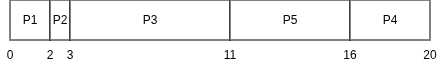
\includegraphics[width=0.8\textwidth]{image3.png}
    \caption{Biểu đồ Gantt lập lịch theo số hiệu ưu tiên cho phép dừng} 
    \label{fig:image3} 
\end{figure}
\noindent Từ biểu đồ Gantt cho lập lịch theo số hiệu ưu tiên cho phép dừng, thời gian chờ trung bình, thời gian phản hồi trung bình, thời gian hoàn thành trung bình và số lần chuyển trạng thái được tính như sau:\\\\
\textbf{Thời gian chờ trung bình}
\begin{itemize}
    \item Thời gian chờ $T_{w1} = (2 - 0) - 2 = 0$
    \item Thời gian chờ $T_{w2} = (3 - 1) - 1 = 1$
    \item Thời gian chờ $T_{w3} = (11 - 3) - 8 = 0$
    \item Thời gian chờ $T_{w4} = (20 - 4) - 4 = 12$
    \item Thời gian chờ $T_{w5} = (16 - 5) - 5 = 6$
    \item Thời gian chờ trung bình $T_w = \frac{0 + 1 + 0 + 12 + 6}{5} = 3.8 (ms)$ 
\end{itemize}

\textbf{Thời gian phản hồi trung bình}
\begin{itemize}
    \item Thời gian phản hồi $T_{res1} = 0 - 0 = 0$
    \item Thời gian phản hồi $T_{res2} = 2 - 1 = 1$
    \item Thời gian phản hồi $T_{res3} = 3 - 3 = 0$
    \item Thời gian phản hồi $T_{res4} = 16 - 4 = 12$
    \item Thời gian phản hồi $T_{res5} = 11 - 5 = 6$
    \item Thời gian phản hồi trung bình $T_{res} = \frac{0 + 1 + 0 + 12 + 6}{5} = 3.8 (ms)$ 
\end{itemize}

\textbf{Thời gian hoàn thành trung bình}
\begin{itemize}
    \item Thời gian hoàn thành $T_{tat1} = 2 - 0 = 2$
    \item Thời gian hoàn thành $T_{tat2} = 3 - 1 = 2$
    \item Thời gian hoàn thành $T_{tat3} = 11 - 3 = 8$
    \item Thời gian hoàn thành $T_{tat4} = 20 - 4 = 16$
    \item Thời gian hoàn thành $T_{tat5} = 16 - 5 = 11$
    \item Thời gian hoàn thành trung bình $T_{tat} = \frac{2 + 2 + 8 + 16 + 11}{5} = 7.8 (ms)$ 
\end{itemize}

\textbf{Số lần chuyển trạng thái của CPU}
Dựa trên các điểm thay đổi tiến trình trên biểu đồ Gantt:
\begin{itemize}
    \item Lần chuyển 1: $P_1 \rightarrow P_2$ tại $t=2$
    \item Lần chuyển 2: $P_2 \rightarrow P_3$ tại $t=3$ (Do $P_3$ có ưu tiên 5 cao nhất)
    \item Lần chuyển 3: $P_3 \rightarrow P_5$ tại $t=11$ (Sau khi $P_3$ xong, $P_5$ ưu tiên 4 cao kế tiếp)
    \item Lần chuyển 4: $P_5 \rightarrow P_4$ tại $t=16$ (Sau khi $P_5$ xong, đến lượt $P_4$ ưu tiên 3)
    \item Tổng số lần chuyển trạng thái: 4
\end{itemize}
\section{Bài tập 2}
\subsection{Đề bài}
Vẽ biểu đồ Gantt và tính thời gian chờ trung bình, thời gian hoàn thành trung bình, thời gian
phản hồi trung bình cho các tiến trình khi sử dụng thuật toán hàng đợi đa cấp.
\begin{table}[H]
    \centering
    \caption{Bảng thống kê tiến trình, thời gian chạy, thời gian đến, thuật toán sử dung để xử lý 7 tiến trình}
    \begin{tabular}{|c|c|c|c|c|}
        \hline
        \textbf{Hàng đợi} & \textbf{Tiến trình} & \textbf{Thời gian chạy} & \textbf{Thời gian đến} & \textbf{Thuật toán} \\
        \hline
        Hàng đợi trước số 1 & $P_{1}$ & 50 & 0 & RR \\
        & $P_{2}$ & 15 & 30 & quantum=20 \\
        & $P_{3}$ & 45 & 30 & \\
        \hline
        Hàng đợi trước số 2 & $P_{4}$ & 40 & 0 & SJF cho phép dùng \\
        & $P_{5}$ & 10 & 120 & \\
        \hline
        Hàng đợi sau & $P_{6}$ & 30 & 60 & FCFS \\
        & $P_{7}$ & 20 & 130 & \\
        \hline
    \end{tabular}
\end{table}
\noindent Biết rằng trình tự ưu tiên các hàng đợi như sau: Hàng đợi trước số 1, Hàng đợi trước số 2,
Hàng đợi sau.
\subsection{Giải bài tập}
Khi sử dụng thuật toán hàng đợi đa cấp, biết rằng trình tự ưu tiên các hàng đợi như sau: Hàng đợi trước số 1, Hàng đợi trước số 2, các tiến trình sẽ được xử lý thể hiện trên biểu đồ Gantt như sau:
\begin{figure}[H]
    \centering 
    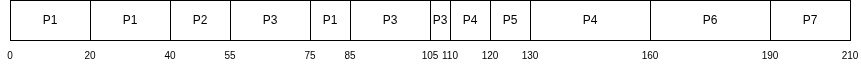
\includegraphics[width=1\textwidth]{image4.png}
    \caption{Biểu đồ Gantt khi sử dụng thuật toán hàng đợi đa cấp} 
    \label{fig:image4} 
\end{figure}
\noindent Từ biểu đồ Gantt khi sử dụng thuật toán hàng đợi đa cấp, thời gian chờ trung bình,
thời gian phản hồi trung bình, thời gian hoàn thành trung bình như sau:
được tính như sau:\\\\
\textbf{Thời gian chờ trung bình}
\begin{itemize}
    \item Thời gian chờ $T_{w1} = (0-0) + (40-20) + (75-60) = 35$ ms
    \item Thời gian chờ $T_{w2} = 55 - 30 - 15 = 10$ ms
    \item Thời gian chờ $T_{w3} = (30-30) + (85-75) + (105-105) = 10$ ms
    \item Thời gian chờ $T_{w4} = (20-0) + (130-120) = 30$ ms
    \item Thời gian chờ $T_{w5} = 120 - 120 = 0$ ms
    \item Thời gian chờ $T_{w6} = 160 - 60 = 100$ ms
    \item Thời gian chờ $T_{w7} = 190 - 130 = 60$ ms
    \item Thời gian chờ trung bình $T_w = \frac{35 + 10 + 10 + 30 + 0 + 100 + 60}{7} \approx 35.0$ (ms)
\end{itemize}

\textbf{Thời gian phản hồi trung bình}
\begin{itemize}
    \item Thời gian phản hồi $T_{res1} = 0 - 0 = 0$ ms
    \item Thời gian phản hồi $T_{res2} = 40 - 30 = 10$ ms
    \item Thời gian phản hồi $T_{res3} = 55 - 30 = 25$ ms
    \item Thời gian phản hồi $T_{res4} = 20 - 0 = 20$ ms
    \item Thời gian phản hồi $T_{res5} = 120 - 120 = 0$ ms
    \item Thời gian phản hồi $T_{res6} = 160 - 60 = 100$ ms
    \item Thời gian phản hồi $T_{res7} = 190 - 130 = 60$ ms
    \item Thời gian phản hồi trung bình $T_{res} = \frac{0 + 10 + 25 + 20 + 0 + 100 + 60}{7} \approx 30.71$ (ms)
\end{itemize}

\textbf{Thời gian hoàn thành trung bình}
\begin{itemize}
    \item Thời gian hoàn thành $T_{tat1} = 85 - 0 = 85$ ms
    \item Thời gian hoàn thành $T_{tat2} = 55 - 30 = 25$ ms
    \item Thời gian hoàn thành $T_{tat3} = 110 - 30 = 80$ ms
    \item Thời gian hoàn thành $T_{tat4} = 160 - 0 = 160$ ms
    \item Thời gian hoàn thành $T_{tat5} = 130 - 120 = 10$ ms
    \item Thời gian hoàn thành $T_{tat6} = 190 - 60 = 130$ ms
    \item Thời gian hoàn thành $T_{tat7} = 210 - 130 = 80$ ms
    \item Thời gian hoàn thành trung bình $T_{tat} = \frac{85 + 25 + 80 + 160 + 10 + 130 + 80}{7} = 81.43$ (ms)
\end{itemize}
\end{document}